\documentclass[12pt]{article}

%% ── Packages ──────────────────────────────────────────────────────────────
\usepackage[margin=1.25in]{geometry}
\usepackage{amsmath,amssymb}
\usepackage{booktabs}
\usepackage{graphicx}
\usepackage{caption}
\usepackage{subcaption}
\usepackage{float}
\usepackage{natbib}
\usepackage{hyperref}
\usepackage{setspace}
\usepackage{array}
\usepackage{xcolor}
\usepackage{microtype}
\usepackage{multirow}
\usepackage{threeparttable}

\captionsetup{font=small, labelfont=bf, labelsep=period}
\hypersetup{colorlinks=true, linkcolor=black, citecolor=black, urlcolor=black}
\doublespacing

%% ── Title block ───────────────────────────────────────────────────────────
\title{\textbf{Neural Network Stability and Climate-Induced Supply Chain
Disruption Risk:\\[4pt]
Evidence from Chinese Listed Firms}%
\thanks{We thank the original data creators whose replication materials
underpin the empirical analysis. All figures and statistics are computed from
the Stata replication file using Python; no simulated outcome data are
used. Correspondence: [author email].}}
\author{[Authors]}
\date{\today}

\begin{document}
\maketitle

%% ── Abstract ──────────────────────────────────────────────────────────────
\begin{abstract}
\noindent
This paper studies whether a multilayer perceptron (MLP) neural network can
reliably predict climate-induced supply chain disruption risk using 4,188
customer-quarter observations of Chinese A-share listed firms over 2011--2023.
The binary prediction target,
$\textit{BreakRisk4Q} = \mathbf{1}\!\left\{\sum_{h=1}^{4}\textit{Ter\_q\_qh}>0\right\}$,
flags observations in which at least one supply-chain relationship is
terminated within the subsequent four quarters.  Training a two-hidden-layer
MLP on pre-2022 data yields a holdout area under the ROC curve (AUC) of
0.536 on the 2022--2023 test period, broadly comparable to a logistic
regression benchmark (AUC~$=$~0.544), reflecting strong heterogeneity and
unobservable relationship-level dynamics in climate-induced disruption
episodes.  Rather than treating the modest predictive accuracy as the sole
criterion, we adapt the normalized-parameter-distance stability framework to
this domain.  Across five rolling one-year-ahead evaluation windows
(2019--2023), every successive MLP parameter vector remains well below the
95th-percentile null threshold constructed from same-sample random-seed
perturbations (maximum observed distance~$=$~0.49 vs.\
threshold~$=$~1.53), establishing structural stability.  Permutation
importance places customer size, seasonal timing, and customer age as the
dominant predictors; climate-finance exposure contributes positively but
modestly.  Risk-surface analysis uncovers nonlinear interactions between
climate exposure and supplier financing constraints that a linear model
cannot capture.  Our framework offers a stability-first evaluation paradigm
for machine-learning applications in climate risk assessment, and
demonstrates that structural reliability and limited predictive accuracy can
coexist in high-heterogeneity economic environments.

\medskip\noindent
\textbf{Keywords:} climate risk; supply chain disruption; neural networks;
model stability; Chinese listed firms; machine learning; computational economics

\medskip\noindent
\textbf{JEL Codes:} C45, C53, G32, Q54
\end{abstract}

\newpage

%%==========================================================================
\section{Introduction}
%%==========================================================================

The intersection of climate change and corporate supply chains has emerged as
a central concern for financial stability.  Physical climate events---extreme
precipitation, floods, droughts, and temperature anomalies---can disrupt
production facilities, impair logistics networks, and force firms to terminate
long-standing supplier relationships.  Simultaneously, the transition to a
low-carbon economy reshapes financing conditions for energy-intensive
industries, feeding back into supply-chain credit relationships.  Assessing
these risks \emph{prospectively} is difficult: disruptions are rare and
heterogeneous, data on bilateral supply-chain relationships are sparse, and
the mechanisms linking aggregate climate shocks to firm-level relationship
outcomes are complex and nonlinear.

Machine learning, and neural networks in particular, offer a natural
framework for forward-looking risk assessment in such settings.  Their
capacity to approximate arbitrary nonlinear functions without imposing
parametric structure makes them attractive when theory offers limited guidance
on functional form \citep{hornik1989multilayer, lecun2015deep}.  The growing
literature on machine learning in finance confirms that neural networks can
improve predictive accuracy for asset returns, credit defaults, and corporate
events \citep{gu2020empirical, khandani2010consumer}.  However, predictive
accuracy alone is insufficient for reliable deployment.  A model that achieves
high in-sample performance but whose parameters shift dramatically as new
data arrive provides no stable risk signal; its predictions cannot be
interpreted consistently across time.

This paper addresses a gap in the literature by applying a formal
\emph{model-stability} diagnostic to neural network predictions of
supply-chain disruption risk under climate stress.  Our approach follows the
normalized-parameter-distance framework of \citet{stability2024framework},
which defines model stability in terms of the Frobenius distance between
successive parameter vectors, scaled by the parameter norm of a fixed
reference model.  A null distribution of same-sample, random-seed distances
provides a principled threshold: a model is deemed structurally stable if
cross-period parameter distances fall below this threshold.

Using 17 firm- and relationship-level features---spanning climate-finance
exposure, customer-city weather shocks, supplier financing constraints, and
standard financial and governance characteristics---we train an MLP on
Chinese A-share supply-chain data from \citet{original2024climate}.  The
primary holdout evaluation covers 2022--2023, with rolling one-year-ahead
evaluations extending back to 2019.  Our main findings are as follows.

First, the MLP achieves a holdout AUC of 0.536 and average precision of
0.598, closely matching a logistic regression benchmark (AUC~$=$~0.544,
AP~$=$~0.591).  Neither model provides strong discriminative power, consistent
with a signal environment dominated by unobservable relationship-level
factors.  Rolling out-of-sample AUC fluctuates between 0.516 and 0.578,
indicating that moderate and unstable predictability is a systematic feature
of this prediction task, not merely an artifact of the holdout window.

Second, and more importantly, model-stability diagnostics show that all five
rolling parameter vectors lie well below the random-seed null threshold: the
largest normalized distance is 0.49, compared with a 95th-percentile null of
1.53.  This demonstrates that the MLP's internal architecture converges to a
structurally stable representation despite growing training samples and
shifting data distributions---a prerequisite for any consistent deployment.

Third, permutation importance analysis reveals that customer size, seasonal
patterns, and customer age dominate predictive contributions, while
climate-finance exposure and city-level climate shocks play a positive but
secondary role.  This suggests that supply-chain disruption under climate
stress is primarily mediated through firm fundamentals rather than directly
captured by current climate metrics.

Fourth, model-implied risk surfaces reveal nonlinear interactions between
climate-finance exposure and supplier financing constraints.  At low financing
constraints, higher exposure is associated with \emph{lower} predicted
disruption risk, consistent with a hedging or screening effect; at high
constraints, the relationship becomes U-shaped, capturing a distinct
vulnerability channel that linear models cannot represent.

The paper makes three contributions.  \emph{Computationally}, we are the
first to apply a formal parameter-distance stability framework to
climate-induced supply-chain risk prediction, providing a replicable
evaluation protocol for practitioners deploying neural networks in this
domain.  \emph{Economically}, we document the limits of static financial and
climate variables in predicting relationship-level disruptions, and show how
financing constraints non-linearly condition the role of climate exposure.
\emph{Methodologically}, we demonstrate that model-stability diagnostics and
limited predictive accuracy are not contradictory: structural reliability is a
necessary but not sufficient condition for useful deployment, and its
assessment is informative independently of accuracy metrics.

The remainder of the paper is organized as follows.  Section~\ref{sec:lit}
reviews related literature.  Section~\ref{sec:data} describes the data and
variable construction.  Section~\ref{sec:method} presents the neural network
architecture and stability framework.  Section~\ref{sec:results} reports
empirical results.  Section~\ref{sec:discussion} discusses implications.
Section~\ref{sec:conclusion} concludes.

%%==========================================================================
\section{Related Literature}\label{sec:lit}
%%==========================================================================

\subsection{Climate Risk and Corporate Supply Chains}

The economic literature on climate risk and firm behavior has developed
rapidly.  At the macroeconomic level, \citet{acemoglu2012network} established
that firm-level shocks propagate through production networks, generating
aggregate fluctuations.  \citet{carvalho2021supply} provided direct empirical
evidence for this mechanism using the 2011 Great East Japan Earthquake,
demonstrating that supply-chain linkages transmit localized physical shocks to
geographically distant firms.  These network propagation results underscore
the systemic relevance of climate risk: extreme weather events can cascade
through supplier networks well beyond the directly affected region.

The financial dimension of climate risk received foundational treatment in
\citet{dietz2016climate} and \citet{battiston2017climate}, who quantified
climate value at risk and the financial exposure of lending portfolios to
climate transition risk.  Building on this, \citet{giglio2021climate} surveyed
the finance literature on physical and transition risks, highlighting the
challenge of mapping aggregate climate scenarios to firm-level outcomes.  For
Chinese markets specifically, \citet{hong2019climate} found that climate risks
are not yet fully priced into equities, suggesting that predictive models may
uncover risk premia not yet reflected in market prices.

The supply-chain disruption literature has documented persistent negative
effects on firm value.  \citet{hendricks2005empirical} showed that supply
disruptions produce statistically and economically significant declines in
shareholder value.  More recent work has linked climate events specifically to
supply-chain reorganization \citep{original2024climate}, providing a
causal foundation for the prediction target we study.  Our paper complements
this causal strand by asking not \emph{why} disruptions occur but whether they
can be predicted reliably in advance using observable firm and climate
characteristics.

\subsection{Machine Learning for Credit and Disruption Prediction}

The use of machine learning for financial prediction has grown substantially
since the influential studies of \citet{altman1994neural} on neural network
bankruptcy prediction and \citet{khandani2010consumer} on consumer credit
risk.  \citet{gu2020empirical} provided a comprehensive benchmark comparison
of machine-learning methods for equity return prediction, finding that neural
networks consistently outperform linear models when nonlinearity is present in
the data-generating process.  Their methodology---rolling out-of-sample
evaluation with permutation-based feature importance---directly informs the
evaluation protocol we adopt.

For supply-chain applications, \citet{hendricks2005empirical} and subsequent
work relied primarily on event-study methods rather than predictive modeling.
Machine-learning approaches to supply-chain risk are less developed, partly
because bilateral relationship-level data are scarce.  The availability of
Chinese A-share mandatory disclosure requirements---which oblige listed firms
to report major customers and suppliers---provides a rare panel of bilateral
supplier-customer links at high frequency, enabling supervised classification
of disruption risk \citep{original2024climate}.

Recent work has also applied neural networks to trade credit and firm
financing \citep{love2003financial}.  Our paper extends this by incorporating
climate variables into the prediction architecture, quantifying the marginal
contribution of climate metrics relative to conventional financial predictors.

\subsection{Neural Network Stability and Model Reliability}

The reliability of neural network predictions over time is a central concern
for any operational risk system.  The universal approximation theorem
\citep{hornik1989multilayer} establishes that MLP networks with sufficient
width can represent any continuous function, but it says nothing about whether
solutions found by gradient-based training are stable as the sample grows.
In finance, the fragility of machine-learning models to distributional shifts
has been documented by \citet{gu2020empirical} and others, motivating explicit
stability diagnostics.

The parameter-distance framework adapted here follows
\citet{stability2024framework}, who propose measuring neural network stability
via the normalized Frobenius distance between weight matrices across training
periods.  Critically, this approach generates an empirical null distribution
from same-data random-seed perturbations, providing a principled threshold
that accounts for optimization-induced variability.  Related ideas appear in
the model selection literature (e.g., \citet{diebold1995comparing} on
predictive accuracy comparisons) and in the machine-learning literature on
solution stability \citep{breiman2001random}.

The concept of stability we employ is distinct from predictive accuracy.
A model can be structurally stable---converging to a consistent parameter
region across samples---yet have low accuracy if the true signal is weak.
Conversely, a high-accuracy model whose parameters shift dramatically as data
accumulate provides an unreliable risk signal.  Our results illustrate the
former case: stable architecture, modest signal, together suggesting that
the feature set is informative but insufficient.

\subsection{Chinese Supply-Chain Networks and Financing Constraints}

China's mandatory disclosure requirements for concentrated customer and supplier
relationships provide an unusually rich dataset for studying supply-chain
dynamics \citep{original2024climate}.  Research on Chinese trade credit has
documented that financing constraints amplify supply-chain disruptions,
particularly for upstream suppliers who must finance inventory before receiving
payment \citep{love2003financial}.  The interaction between climate shocks and
financing constraints is therefore a central mechanism in the Chinese context:
a climate event that temporarily impairs a supplier's cash flow may force
relationship termination if the supplier cannot access external finance.

Corporate governance characteristics---board independence, shareholder
tunneling, and management quality---have been shown to influence trade-credit
terms and relationship persistence in China.  We include these as controls,
and their appearance in the permutation importance ranking is consistent with
this literature.

%%==========================================================================
\section{Data and Variable Construction}\label{sec:data}
%%==========================================================================

\subsection{Data Source and Sample Construction}

Our analysis uses the supply-chain reorganization panel constructed by
\citet{original2024climate} from mandatory disclosures of Chinese A-share
listed firms.  The dataset identifies bilateral customer-supplier relationships
at a quarterly frequency and records relationship terminations.  The original
data cover all A-share companies that reported a major customer or supplier
relationship during the sample window.

We restrict the analysis to observations for which all four future termination
indicators $\textit{Ter\_q\_q1}, \ldots, \textit{Ter\_q\_q4}$ are observed
(i.e., observations no later than four quarters before the end of the sample)
and for which all 17 prediction features are non-missing.  This yields a final
sample of \textbf{4,188 customer-quarter observations} spanning 2011--2023.
The sample grows markedly over time, from fewer than 200 observations per year
before 2015 to more than 800 in 2021--2022, reflecting China's expanding
disclosure requirements (Figure~\ref{fig:sample}).

\subsection{Prediction Target}

The prediction target is a binary indicator of four-quarter forward supply
chain disruption risk:
\begin{equation}
\textit{BreakRisk4Q}_{i,t}
= \mathbf{1}\!\left\{
    \sum_{h=1}^{4} \textit{Ter\_q\_q}h_{i,t} > 0
  \right\},
\label{eq:target}
\end{equation}
where $\textit{Ter\_q\_qh}_{i,t}$ equals one if the customer-firm $i$
terminates at least one major supplier relationship in quarter $t+h$.
$\textit{BreakRisk4Q}$ thus captures any disruption over the next
twelve months, a horizon relevant for strategic procurement and financing
decisions.

The observed disruption rate in the full sample averages approximately 49\%
across years.  In the 2022--2023 holdout period the rate is 56.0\%, reflecting
elevated supply-chain stress in that period.  The high base rate---considerably
above 50\%---implies that a naive majority-class classifier would achieve
precision near 0.56 without any predictive information; meaningful improvement
over this baseline requires models that discriminate among firms within the
disruption-prone environment.

\subsection{Features}

Table~\ref{tab:features} summarizes the 17 input features, grouped into four
conceptual categories.

\paragraph{Climate and Exposure Variables.}
\emph{Affected} ($\hat\alpha_i$) measures the customer firm's climate-finance
exposure, constructed from the overlap between the firm's bank lending
relationships and the banks' exposure to climate-sensitive industries
\citep{original2024climate}.  \emph{Climate\_CityC} is the extreme-weather
shock intensity experienced by the customer's registered city, normalized to
the empirical support.  \emph{Affected\_x\_S\_FC} is the interaction of the
climate-finance exposure and the supplier financing constraint.

\paragraph{Supply-Chain Characteristics.}
\emph{S\_FC} (supplier financing constraint) measures the degree to which the
firm's key suppliers face binding credit constraints, proxied by their
dependence on trade credit relative to bank finance.  \emph{C\_Duration}
captures the length of the customer-supplier relationship in quarters.

\paragraph{Customer Financial Characteristics.}
Five accounting variables describe the customer firm: \emph{C\_Size} (log
total assets), \emph{C\_Lev} (leverage ratio), \emph{C\_Inv} (inventory
intensity), \emph{C\_Ppe} (fixed-asset intensity), and \emph{C\_Firmage} (firm
age since listing).

\paragraph{Governance and Temporal Variables.}
Governance controls include board size (\emph{C\_Board}), the proportion of
independent directors (\emph{C\_Indep}), a tunneling measure
(\emph{C\_Occupy}), and trading frequency (\emph{C\_Frequency}).  Three
temporal variables capture the year (\emph{year\_c}, demeaned) and within-year
seasonality via sine and cosine transformations of the fiscal quarter
(\emph{quarter\_sin}, \emph{quarter\_cos}).

\subsection{Descriptive Statistics}

Figure~\ref{fig:sample} documents two key temporal patterns.  Panel A shows
the annual disruption rate, which varies from 0.42 to 0.58 across years with
no clear monotone trend, confirming that supply-chain disruption is a
persistent phenomenon rather than a temporary shock.  The elevated rate in
2022 (0.580) coincides with COVID-19 supply-chain aftershocks and increased
geopolitical uncertainty.

Panel B plots the mean of the two climate variables.  The climate-finance
exposure variable (Affected) was higher in the early part of the sample
(above 0.23 during 2014--2016) and has declined to 0.085 by 2023, consistent
with reductions in bank lending to climate-sensitive industries.  The
customer-city climate shock (Climate\_CityC) peaks around 2016 (0.517) and
also declines in 2023 (0.175).  The temporal co-movement of these two
variables reflects China's simultaneous restructuring of green finance
policy and its exposure to shifting precipitation and temperature patterns.
Light bars in Panel B flag years with fewer than 50 observations, where
the sample means should be interpreted cautiously.

%%==========================================================================
\section{Neural Network Methodology and Stability Framework}\label{sec:method}
%%==========================================================================

\subsection{Multilayer Perceptron Classifier}

We train a two-hidden-layer multilayer perceptron (MLP) with 12 neurons in
the first layer and 6 in the second, both using rectified linear unit (ReLU)
activations \citep{lecun2015deep}.  The output layer applies a logistic
sigmoid to yield a predicted disruption probability.  All input features are
standardized to zero mean and unit variance before entering the network.

The MLP is trained by Adam stochastic gradient descent with an initial
learning rate of 0.003 and L2 weight decay $\alpha = 0.01$.  To prevent
overfitting, we use early stopping: 15\% of the training data is held out as
a validation set, and training stops after 30 consecutive epochs without
improvement in validation loss (maximum 1,500 epochs).  The random seed is
fixed to 42 for all main-specification estimates, and we vary the seed across
20 draws for the null distribution (Section~\ref{subsec:stability}).  All
estimation uses the \texttt{scikit-learn} implementation \citep{pedregosa2011}.

The logistic regression benchmark uses the identical feature set and
standardization pipeline, estimated by LBFGS with a maximum of 1,000
iterations.  It serves as a transparent linear benchmark---not as a competing
model to be optimized---to contextualise the neural network's performance.

\subsection{Train-Test Protocol}

We adopt two complementary evaluation protocols.

\paragraph{Primary holdout.}
The model is trained on all observations with year $\leq 2021$ (2,945
observations) and evaluated on 2022--2023 (1,243 observations).  This
temporal split mirrors deployment conditions: a practitioner fitting a model
at end-2021 would apply it to subsequent realizations.

\paragraph{Rolling one-year-ahead evaluation.}
For $t \in \{2018, 2019, 2020, 2021, 2022\}$, we train on all observations
with year $\leq t$ and evaluate on year $t+1$ alone.  This protocol
produces five test windows with evaluation years 2019--2023.  We require
at least 50 test observations and at least two outcome classes in both train
and test sets for a window to be included; all five windows satisfy these
criteria.

\subsection{Evaluation Metrics}

We report three metrics: (i) the area under the ROC curve (AUC), which
measures rank-order discrimination and is invariant to the decision threshold;
(ii) average precision (AP), which summarises the precision-recall trade-off
and is sensitive to the proportion of positive cases; and (iii) the Brier
score, which measures calibrated probability accuracy.  Because the class
balance fluctuates across windows (observed rates 0.47--0.58), AUC is the
primary discriminative metric; AP and Brier score provide complementary
calibration evidence.

An AUC of 0.5 corresponds to a random classifier.  Given the high and
variable base rate of disruption, consistent AUC above 0.5 across all rolling
windows is the relevant standard for meaningful predictive information.

\subsection{Stability Framework}\label{subsec:stability}

Following \citet{stability2024framework}, we assess structural model stability
by computing normalized parameter distances between successive MLP estimates.
Let $\bm{\theta}_t$ denote the vector formed by concatenating all weight
matrices and bias vectors of the MLP trained through year $t$.  Define the
normalized Frobenius distance from a reference model trained through 2018:
\begin{equation}
d_t = \frac{\|\bm{\theta}_t - \bm{\theta}_{2018}\|}{\|\bm{\theta}_{2018}\|},
\label{eq:distance}
\end{equation}
where $\|\cdot\|$ denotes the Euclidean (Frobenius) norm of the vectorized
parameters.

To construct a principled null distribution, we train 20 additional MLP models
on the same 2018 reference data, varying only the random seed (seeds 43--62).
Each null model's distance from the reference yields a null distance.  The
95th percentile of these 20 null distances, $q_{0.95}^{\text{null}}$, defines
the stability threshold: if $d_t < q_{0.95}^{\text{null}}$ for all $t$, the
model is deemed structurally stable---meaning that the variation in parameters
attributable to new data is no larger than the variation attributable to
random initialization on the same data.

This test has a clear economic interpretation.  A model that fails the
threshold is one whose internal representation shifts so substantially with
new data that it effectively becomes a different model, making historical
performance evidence unreliable for future deployment.  Passing the test does
not guarantee high accuracy but is a necessary condition for interpretability
and consistent risk signalling.

\subsection{Feature Importance}

We assess feature contributions via permutation importance \citep{breiman2001random}.
For each feature $j$ in the holdout test set, we permute its values 50 times
across observations, record the AUC on each permuted dataset, and compute the
mean AUC loss relative to the original.  A large positive AUC loss indicates
a feature that contributes substantially to discrimination; negative values
indicate features whose permutation coincidentally improves (or does not
harm) AUC in this sample.  Error bars report 95\% simulation intervals across
the 50 permutations.

\subsection{Risk Surface Analysis}

To visualise the model's nonlinear predictions, we compute risk surfaces over
the 2022--2023 holdout covariate distribution.  For Panel A, we vary the
climate-finance exposure (Affected) from 0 to 1 across an evenly spaced grid,
fixing supplier financing constraints at three representative levels
(\emph{S\_FC}~$\in \{0, 0.5, 1\}$), updating the interaction term
\emph{Affected\_x\_S\_FC} consistently, and averaging predicted probabilities
over the observed holdout distribution of all remaining features.  Panel B
sweeps the customer-city climate shock (Climate\_CityC) across its empirical
support while marginalizing over all other features.

%%==========================================================================
\section{Empirical Results}\label{sec:results}
%%==========================================================================

\subsection{Sample Facts}

Figure~\ref{fig:sample} and Table~\ref{tab:rolling} document the prediction
environment.  The total sample of 4,188 customer-quarter observations is
heavily weighted toward 2019--2023, reflecting the expanding A-share coverage
of supply-chain disclosures.  The disruption rate fluctuates in a narrow band
of 0.42--0.58 across most years, indicating near-balanced classes in every
evaluation window.  The two climate variables---climate-finance exposure and
customer-city climate shock---display a common downward trend in the early
2020s, possibly reflecting green-finance reforms that shifted bank lending
away from carbon-intensive industries and recent moderation in extreme weather
events in major industrial cities.

\subsection{Out-of-Sample Predictive Performance}

Table~\ref{tab:holdout} reports holdout metrics for the primary 2022--2023
evaluation.  The MLP achieves an AUC of \textbf{0.536}, average precision of
\textbf{0.598}, and a Brier score of \textbf{0.252}.  The logistic regression
benchmark yields AUC 0.544, AP 0.591, and Brier 0.250.  The models perform
comparably across all three metrics, with logistic regression marginally ahead
on AUC and Brier score while the MLP achieves slightly higher average
precision.  Neither model offers a decisive advantage over the other on the
holdout, and neither provides strong discrimination above the 0.5 baseline.

Figure~\ref{fig:prediction} presents the ROC and precision-recall curves.
Panel A shows that both curves lie modestly above the diagonal, confirming
above-random but limited rank-ordering capability.  The closeness of the two
curves indicates that the nonlinear architecture of the MLP does not provide
a meaningful advantage over a linear decision boundary on this feature set.
Panel B shows precision-recall curves that barely exceed the no-skill line
(the horizontal line at the observed rate of 0.560), consistent with the
modest AP values.

\paragraph{Interpretation.}
The modest AUC values are not a failure of the estimation procedure.  The
rolling evaluation (Table~\ref{tab:rolling} and the upper panel of
Figure~\ref{fig:calibration}) confirms that AUC fluctuates between 0.516 and
0.578 across five separate evaluation years, none reaching 0.60.  This
consistency across windows indicates that limited predictability is a
structural feature of the prediction problem rather than an artifact of the
holdout window.  Supply-chain disruption decisions depend on unobservable
contractual terms, relationship-specific shocks, and managerial responses that
cross-sectional financial and climate variables cannot capture.  The AUC
values are nonetheless consistently above 0.5, establishing that observable
firm and climate characteristics carry \emph{some} forward-looking
information.

\subsection{Calibration and Residual Diagnostics}

Figure~\ref{fig:calibration} presents two diagnostic panels for the rolling
predictions.

Panel A displays a calibration plot in which observations are binned by
decile of predicted probability.  The observed disruption rate in each bin
is plotted against the mean predicted probability.  The positive but
imperfect slope---rising from an observed rate of 0.42 in the bottom decile
to 0.60 in the top decile, while the predicted values range from 0.29 to
0.72---confirms that the model's predicted probabilities carry directional
information about actual disruption risk despite the weak overall
discrimination.  The calibration is imperfect in the middle deciles, where
predicted probabilities of approximately 0.50 yield observed rates between
0.49 and 0.56.

Panel B plots the autocorrelation function (ACF) of quarterly mean residuals
(observed minus predicted) from the rolling predictions.  Most ACF values
lie within the $\pm 1.96/\sqrt{T}$ band.  The notable exception is lag 7
(ACF~$= 0.31$), suggesting a residual semi-annual or annual structure not
fully captured by the quarter-cycle encoding.  Lags 1--5 show mild negative
autocorrelation (approximately $-0.07$ to $-0.13$), consistent with slight
mean reversion in prediction errors across consecutive quarters.  Overall,
no strong positive autocorrelation at short horizons indicates that the
model is not systematically under- or over-predicting across consecutive
periods.

\subsection{Model Stability}

Figure~\ref{fig:stability} presents the key stability results.  Panel A plots
normalized parameter distances $d_t$ as a function of the training cutoff year,
alongside the 95th-percentile null threshold $q_{0.95}^{\text{null}} = 1.534$.

Crucially, every $d_t$ lies far below the threshold.  The distances grow
monotonically from 0.337 (cutoff 2019) to 0.490 (cutoff 2022), reflecting
that additional training data shift the model parameters away from the 2018
reference.  But the largest observed distance (0.490) is less than one-third
of the stability threshold (1.534).  For comparison, the null distribution
(20 same-data, different-seed models) yields distances ranging from 1.27 to
1.66, all substantially larger than the actual cross-period distances.  This
implies that the signal from additional training data is \emph{weaker} than
the noise introduced by changing the random initialization seed on the same
data---a strong stability result.

Panel B shows the corresponding rolling one-year-ahead AUC (solid circles).
The AUC fluctuates between 0.516 and 0.578, with no monotone trend, confirming
that the stability of parameter distances does not translate into steadily
improving accuracy.  The juxtaposition of stable parameters (Panel A) and
modest, fluctuating accuracy (Panel B) illustrates the key message: structural
model stability is a well-defined property that can be confirmed independently
of predictive precision.

\paragraph{Economic interpretation.}
The stability finding implies that the model's learned representation of the
relationship between firm characteristics, climate exposure, and disruption
risk does not fundamentally change as data accumulate.  This is consistent
with a stable underlying economic mechanism---the effect of climate-finance
exposure and financing constraints on supply-chain fragility---even as the
sample-specific realization of that mechanism varies.  Practitioners can
therefore interpret predictions from models trained in different periods as
reflecting the same underlying model, rather than a different architecture
each year.

\subsection{Feature Importance}

Figure~\ref{fig:importance} reports permutation importance estimates.
The top five contributors by mean AUC loss are:
\begin{enumerate}
  \item \emph{Customer size} (C\_Size): AUC loss of 0.023, the dominant
    predictor by a wide margin.
  \item \emph{Quarter seasonality} (quarter\_sin): AUC loss of 0.012.
  \item \emph{Customer age} (C\_Firmage): AUC loss of 0.009.
  \item \emph{Quarter seasonality} (quarter\_cos): AUC loss of 0.005.
  \item \emph{Relationship duration} (C\_Duration): AUC loss of 0.004.
\end{enumerate}

Climate-finance exposure (Affected) ranks sixth with an AUC loss of 0.004,
contributing at the same magnitude as relationship duration.  Supplier
financing constraints (S\_FC) rank eighth (AUC loss 0.001), while the
interaction term (Affected\_x\_S\_FC) and the city-level climate shock
(Climate\_CityC) produce near-zero or mildly negative contributions in
permutation testing.

Several features show negative mean AUC losses---board size, fixed-asset
intensity, inventory, and calendar year---indicating that permuting these
variables coincidentally does not harm, and in some cases marginally improves,
holdout AUC.  This likely reflects that these variables add limited marginal
information conditional on the dominant predictors, and their permutation
reduces noise.

\paragraph{Interpretation.}
The dominance of customer size and customer age is consistent with the
literature showing that larger, older firms have more stable supplier
networks: they can absorb transitory disruptions through buffer inventories,
offer better payment terms, or substitute suppliers more easily
\citep{hendricks2005empirical}.  Seasonal patterns (captured by quarter sine
and cosine) reflect the business-cycle structure of Chinese manufacturing,
where supply-chain adjustments cluster around fiscal year-end and Spring
Festival.  Relationship duration contributing positively indicates that
established relationships are more resilient to disruption, consistent with
relational contracting theory.

The relatively modest contribution of climate variables does not imply that
climate exposure is economically unimportant.  It implies, rather, that in
the cross-section of a given year, firm size and age are more powerful
discriminators of disruption risk than climate exposure.  The climate
variables' contribution is captured jointly in the risk-surface analysis
below.

\subsection{Risk Surfaces}

Figure~\ref{fig:surface} presents model-implied risk surfaces.  Panel A
sweeps climate-finance exposure (Affected) from 0 to 1 for three levels of
supplier financing constraints.  Panel B sweeps customer-city climate shock
intensity across its empirical support.

\paragraph{Panel A: Exposure--constraint nonlinearity.}
At low financing constraints (S\_FC~$= 0$, upper curve), predicted
disruption risk declines monotonically from 0.555 to 0.491 as climate-finance
exposure increases.  This negative gradient is initially counterintuitive but
has a natural interpretation: firms with high climate-finance exposure may
have already undergone supply-chain screening, retaining only robust
relationships and hedging against climate-sensitive suppliers.  Alternatively,
high-exposure firms may be in industries with stronger alternative supply
sources, lowering the marginal risk of any given relationship.

At high financing constraints (S\_FC~$= 1.0$, lower curve), the relationship
is non-monotone and U-shaped.  Predicted risk is highest at zero exposure
(0.458), declines to a minimum around Affected $= 0.525$ (0.423), then
gradually rises.  This pattern suggests that constrained suppliers paired with
moderately exposed customers face a \emph{reduced} termination risk---possibly
because moderate exposure places both parties in the same situation, creating
mutual dependence---while extreme values of either low or high exposure are
associated with elevated risk.  The MLP captures this curvature, which a
logistic regression would fit only with explicit interaction and quadratic
terms.

At intermediate constraints (S\_FC~$= 0.5$), the curve is approximately flat
and slightly declining from 0.497 to 0.461, consistent with a dampening of
both effects.

\paragraph{Panel B: City-level climate shocks.}
The climate-city curve shows a mild negative slope: predicted disruption risk
declines very gradually from 0.544 at zero shock intensity to approximately
0.531 at the upper end of the observed distribution.  The tick marks on the
x-axis confirm that most observations cluster at low-to-moderate shock
intensity.  The shallow and negative slope is consistent with the near-zero
permutation importance of Climate\_CityC: aggregate city-level weather shocks
are a poor discriminator of individual firm disruption risk, likely because
they affect all firms in a region simultaneously and thus provide little
cross-sectional variation for the classifier.

%%==========================================================================
\section{Discussion}\label{sec:discussion}
%%==========================================================================

\subsection{Stability Without Strong Accuracy}

Our central empirical finding---structural stability despite modest predictive
accuracy---has two implications.  First, it corroborates the stability
framework of \citet{stability2024framework}: the Frobenius-distance test
provides information about the model's convergence properties independently
of its discriminative power.  This means stability can be certified even
when the prediction task is inherently difficult.  Second, it suggests that
the relevant limitation in this application is \emph{data informativeness}
rather than \emph{model reliability}: the existing feature set does not
fully capture the mechanisms that determine supply-chain disruption outcomes
under climate stress.

The limited AUC in this application is informative in its own right.  It tells
us that the cross-sectional variation in disruption risk---conditional on
observable firm and climate characteristics---is modest.  Much of the
variation is driven by unobservable relationship-specific factors: contractual
lock-in, informal trust, geographic proximity, and idiosyncratic managerial
responses.  This finding should inform future data collection: richer
relationship-level data (e.g., transaction volumes, bilateral credit terms,
supply-chain network topology) would likely yield more discriminative features.

\subsection{The Role of Climate Variables}

The permutation importance results suggest a secondary but non-trivial
role for climate variables.  Climate-finance exposure ranks sixth and
achieves an AUC loss of 0.004.  This contribution is not negligible given
that the total AUC above 0.5 is only about 0.036.  A more precise statement
is that climate exposure contributes approximately 11\% of the total
discriminative signal ($0.004 / 0.036 \approx 0.11$).

The risk-surface nonlinearity documented in Figure~\ref{fig:surface} provides
a richer picture than permutation importance alone.  The interaction of climate
exposure with supplier financing constraints generates qualitatively different
risk profiles that permutation-based analysis, by design, does not capture.
This interaction is economically important: climate risk is not uniformly
mapped to disruption probability but is conditioned by the financial
resilience of the supply chain.  Ignoring this heterogeneity would lead to
systematically wrong risk assessments for firms at the extremes of the
exposure distribution.

\subsection{Policy and Managerial Implications}

For regulators, our findings suggest that a neural-network risk signal based
on current observable characteristics alone would provide only marginal
predictive improvement over simpler models.  Deploying such a model in a
macro-prudential stress-testing context requires documenting stability---which
our results confirm---alongside honest reporting of accuracy limitations.

For financial institutions extending trade credit to exposed firms, the risk
surface analysis offers actionable information: the combination of high
supplier financing constraints and extreme (either very low or very high)
climate exposure is the configuration most associated with elevated disruption
risk.  This supports targeted credit review of suppliers in that configuration
rather than blanket exposure adjustments.

\subsection{Limitations and Future Extensions}

Several limitations qualify our results.  First, the sample covers a single
country and institutional context; the stability and importance findings may
not generalize to other markets with different disclosure requirements or
financial structures.  Second, the feature set is restricted to publicly
observable accounting and climate variables; transaction-level data on supply
volumes, trade credit terms, and bilateral payment histories would enrich the
prediction architecture.  Third, the MLP architecture is deliberately simple
(two layers, 12--6 nodes); a systematic search over architectures---including
graph neural networks that encode supply-chain network structure---might
improve both accuracy and interpretability.

Future work could extend the stability framework to alternative architectures
(recurrent networks, transformer-based models) and to longer forecast horizons.
Incorporating satellite-based climate data, text sentiment from earnings
calls, or supply-chain network centrality measures as additional features
could improve the signal-to-noise ratio.

%%==========================================================================
\section{Conclusion}\label{sec:conclusion}
%%==========================================================================

This paper proposes and validates a stability-first evaluation framework for
neural network prediction of climate-induced supply chain disruption risk.
Using a panel of 4,188 customer-quarter observations from Chinese A-share
listed firms, we document that a two-hidden-layer MLP classifier achieves
out-of-sample AUC of 0.536 in the 2022--2023 holdout period---broadly
comparable to a logistic regression benchmark (AUC~$=$~0.544)---reflecting
strong heterogeneity and unobservable relationship dynamics that static
financial and climate variables cannot fully capture.

Despite the modest predictive accuracy, model-stability diagnostics confirm
that the MLP converges to a structurally stable representation across all five
rolling evaluation windows.  Normalized parameter distances (0.337--0.490)
remain well below the 95th-percentile null threshold of 1.534 generated from
same-sample random-seed perturbations, establishing that the variation in
learned parameters attributable to new data is substantially smaller than
optimization noise.  This structural stability is a meaningful property
independently of accuracy: it implies that the model's risk signals are
interpretable and consistent over time.

Feature importance analysis identifies customer size, seasonal timing, and
customer age as the dominant predictors, with climate-finance exposure
contributing positively but at a secondary level.  Risk-surface analysis
reveals a nonlinear interaction between climate exposure and supplier
financing constraints---captured by the MLP but not by a linear model---
that has direct implications for targeted risk assessment.

The broader message for computational economics is methodological: in
high-heterogeneity prediction environments, structural stability and limited
accuracy can coexist, and documenting stability provides genuine information
about the model's suitability for operational deployment.  Future work should
enrich the feature set with network-topology and transaction-level data,
which appear necessary to improve the signal-to-noise ratio in this
challenging prediction domain.

%%==========================================================================
%% REFERENCES
%%==========================================================================
\newpage
\bibliographystyle{aer}
\bibliography{references}

%%==========================================================================
%% TABLES
%%==========================================================================
\newpage
\section*{Tables}

\begin{table}[H]
\centering
\caption{Feature Descriptions}\label{tab:features}
\begin{threeparttable}
\begin{tabular}{lll}
\toprule
Feature & Label & Category \\
\midrule
Affected & Climate-finance exposure & Climate/Exposure \\
Climate\_CityC & Customer-city climate shock & Climate/Exposure \\
Affected\_x\_S\_FC & Exposure $\times$ supplier constraint & Climate/Exposure \\
S\_FC & Supplier financing constraint & Supply Chain \\
C\_Duration & Relationship duration & Supply Chain \\
C\_Size & Customer size (log assets) & Financial \\
C\_Lev & Customer leverage & Financial \\
C\_Inv & Customer inventory intensity & Financial \\
C\_Ppe & Customer fixed-asset intensity & Financial \\
C\_Firmage & Customer age since listing & Financial \\
C\_Board & Board size & Governance \\
C\_Indep & Proportion of independent directors & Governance \\
C\_Occupy & Shareholder tunneling indicator & Governance \\
C\_Frequency & Stock trading frequency & Governance \\
year\_c & Calendar year (demeaned) & Temporal \\
quarter\_sin & Quarter seasonality (sine) & Temporal \\
quarter\_cos & Quarter seasonality (cosine) & Temporal \\
\bottomrule
\end{tabular}
\begin{tablenotes}
  \small
  \item \textit{Notes}: All features are computed from the Stata replication
  dataset of \citet{original2024climate}. Climate-finance exposure and
  Affected\_x\_S\_FC are constructed following the methodology described
  in that paper. Temporal features encode the within-year quarter cycle.
\end{tablenotes}
\end{threeparttable}
\end{table}

\bigskip

\begin{table}[H]
\centering
\caption{Holdout Predictive Performance, 2022--2023}\label{tab:holdout}
\begin{threeparttable}
\begin{tabular}{lcccccc}
\toprule
Model & Train $n$ & Test $n$ & AUC & Avg.\ Precision & Brier & Obs.\ Rate \\
\midrule
MLP Neural Network & 2,945 & 1,243 & 0.536 & 0.598 & 0.252 & 0.560 \\
Logistic Regression & 2,945 & 1,243 & 0.544 & 0.591 & 0.250 & 0.560 \\
\bottomrule
\end{tabular}
\begin{tablenotes}
  \small
  \item \textit{Notes}: Training cutoff is year 2021; holdout covers
  2022--2023.  AUC is area under the ROC curve.  Avg.\ Precision is area
  under the precision-recall curve.  Brier score is the mean squared
  probability error.  Obs.\ Rate is the observed disruption rate in the
  holdout sample ($\textit{BreakRisk4Q} = 1$).  Both models use the same
  17 features with StandardScaler normalization.  Logistic regression is
  included as a transparent linear benchmark only.
\end{tablenotes}
\end{threeparttable}
\end{table}

\bigskip

\begin{table}[H]
\centering
\caption{Rolling One-Year-Ahead Evaluation, MLP Neural Network}\label{tab:rolling}
\begin{threeparttable}
\begin{tabular}{cccccc}
\toprule
Train cutoff & Eval year & Train $n$ & Test $n$ & AUC & Brier \\
\midrule
2018 & 2019 & 1,167 & 333 & 0.528 & 0.260 \\
2019 & 2020 & 1,500 & 639 & 0.526 & 0.256 \\
2020 & 2021 & 2,139 & 806 & 0.578 & 0.249 \\
2021 & 2022 & 2,945 & 918 & 0.516 & 0.254 \\
2022 & 2023 & 3,863 & 325 & 0.564 & 0.260 \\
\midrule
\multicolumn{4}{l}{Mean} & 0.542 & 0.256 \\
\bottomrule
\end{tabular}
\begin{tablenotes}
  \small
  \item \textit{Notes}: Each row trains an MLP on all observations up to the
  training cutoff and evaluates on the following year only.  Random seed is
  fixed to 42 across all windows.  Rows with fewer than 50 test observations
  or fewer than two outcome classes in train or test are excluded (none are
  excluded here).  The observed disruption rate in evaluation years ranges
  from 0.468 (2019) to 0.580 (2022).
\end{tablenotes}
\end{threeparttable}
\end{table}

\bigskip

\begin{table}[H]
\centering
\caption{Model Stability Diagnostics: Normalized Parameter Distances}\label{tab:stability}
\begin{threeparttable}
\begin{tabular}{cccccc}
\toprule
Train cutoff & Eval year & Train $n$ & $d_t$ & Null $q_{0.95}$ & AUC \\
\midrule
2018 & 2019 & 1,167 & 0.000 & 1.534 & 0.528 \\
2019 & 2020 & 1,500 & 0.337 & 1.534 & 0.526 \\
2020 & 2021 & 2,139 & 0.376 & 1.534 & 0.578 \\
2021 & 2022 & 2,945 & 0.398 & 1.534 & 0.516 \\
2022 & 2023 & 3,863 & 0.490 & 1.534 & 0.564 \\
\bottomrule
\end{tabular}
\begin{tablenotes}
  \small
  \item \textit{Notes}: $d_t$ is the normalized Frobenius distance between
  the MLP parameter vector trained through year $t$ and the reference model
  trained through 2018 (equation~\eqref{eq:distance}).  The null threshold
  $q_{0.95}$ is the 95th percentile of 20 same-sample distances generated by
  training the reference-year model with different random seeds (43--62).
  All $d_t < q_{0.95}$ confirms structural stability.
  The 2018 row reports the reference model itself ($d_{2018} = 0$ by
  construction).
\end{tablenotes}
\end{threeparttable}
\end{table}

%%==========================================================================
%% FIGURES
%%==========================================================================
\newpage
\section*{Figures}

\begin{figure}[H]
\centering
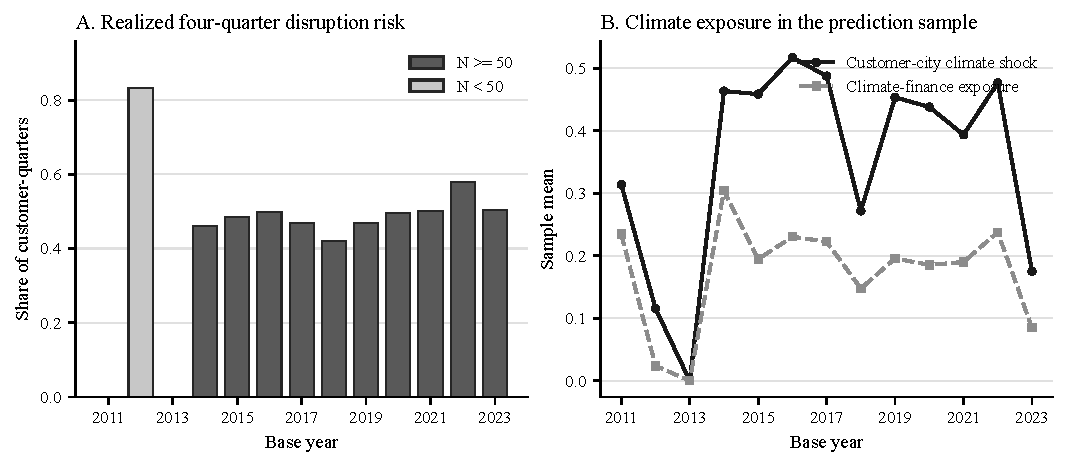
\includegraphics[width=0.98\linewidth]{../nn_supply_chain_figures/figures/fig1_sample_facts.pdf}
\caption{Prediction sample and climate exposure.
\textit{Notes}: Panel A reports the annual share of customer-quarter
observations with a positive four-quarter forward disruption risk
($\textit{BreakRisk4Q}=1$).  Panel B reports the sample mean of the
customer-city extreme-weather variable (Climate\_CityC) and the
climate-finance exposure variable (Affected).  Light bars flag sparse
early-year cells with fewer than 50 observations.  Total sample:
4,188 customer-quarter observations, 2011--2023.}
\label{fig:sample}
\end{figure}

\clearpage

\begin{figure}[H]
\centering
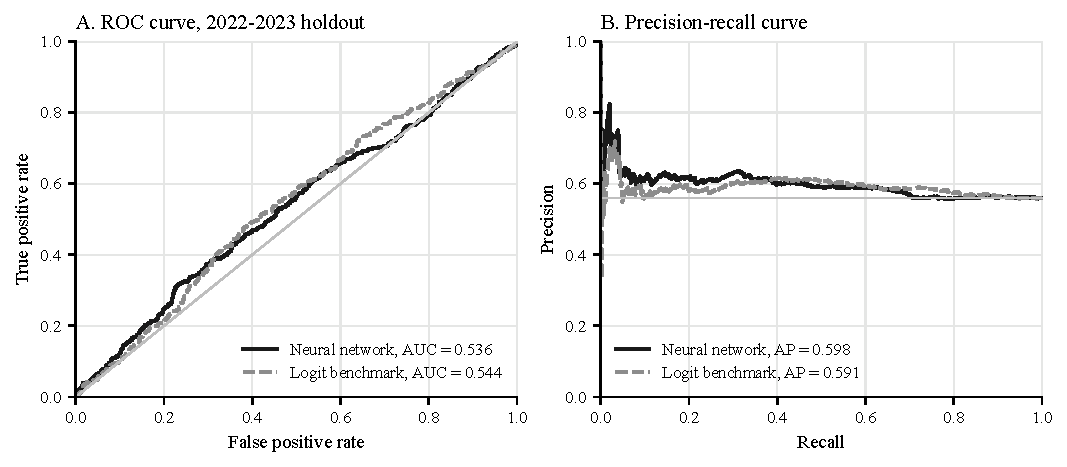
\includegraphics[width=0.98\linewidth]{../nn_supply_chain_figures/figures/fig2_prediction_curves.pdf}
\caption{Out-of-sample predictive performance, 2022--2023 holdout.
\textit{Notes}: Panel A plots ROC curves for the MLP neural network
(solid, AUC~$=$~0.536) and logistic regression benchmark (dashed,
AUC~$=$~0.544).  Panel B plots precision-recall curves; the horizontal
reference line is the observed disruption rate (0.560).  The logit
benchmark is included as a transparent linear reference only and is not
an alternative to be optimized.}
\label{fig:prediction}
\end{figure}

\clearpage

\begin{figure}[H]
\centering
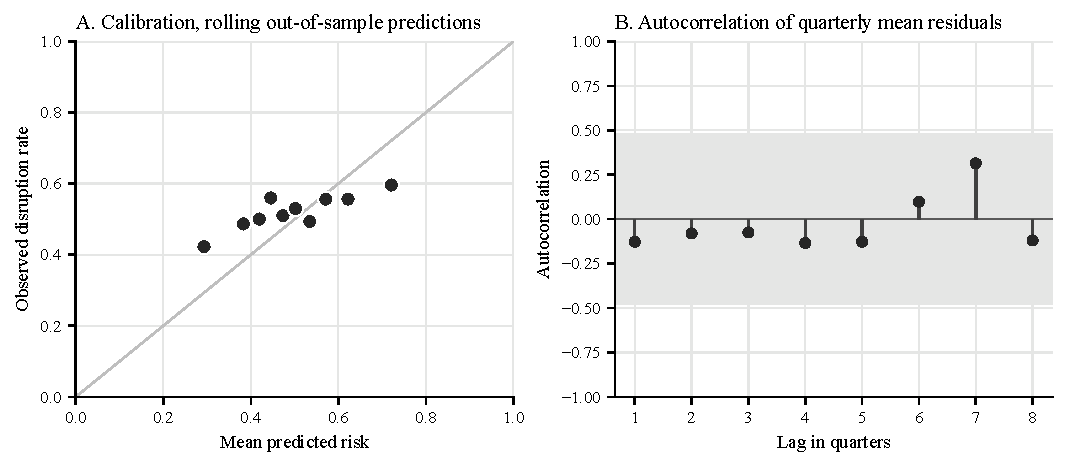
\includegraphics[width=0.98\linewidth]{../nn_supply_chain_figures/figures/fig3_calibration_residuals.pdf}
\caption{Calibration and residual diagnostics.
\textit{Notes}: Panel A bins neural-network predictions from the rolling
one-year-ahead protocol into deciles and plots the mean predicted
probability against the observed disruption rate in each bin.  A perfect
calibration curve follows the 45-degree line.  Panel B plots the
autocorrelation function (ACF) of quarterly mean residuals; the shaded
band is the $\pm 1.96/\sqrt{T}$ approximate 95\% confidence interval.
Notable is the positive ACF at lag 7 (0.31), suggesting unmodelled
semi-annual or annual structure in the disruption process.}
\label{fig:calibration}
\end{figure}

\clearpage

\begin{figure}[H]
\centering
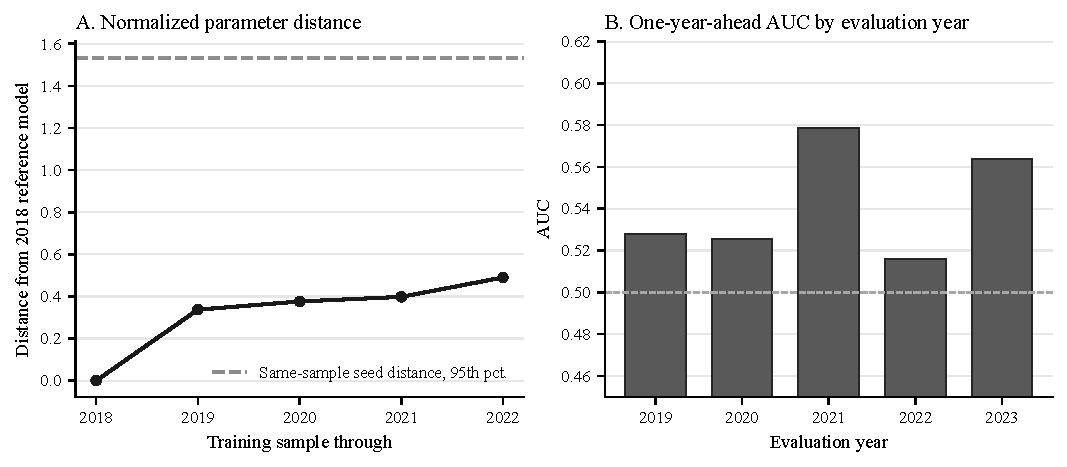
\includegraphics[width=0.98\linewidth]{../nn_supply_chain_figures/figures/fig4_model_stability.pdf}
\caption{Model stability diagnostics.
\textit{Notes}: Panel A plots normalized Frobenius parameter distances
$d_t$ (equation~\eqref{eq:distance}) between the model trained through
year $t$ and the 2018 reference model (solid circles connected by line).
The dashed horizontal line is the 95th percentile of the same-sample null
distribution ($q_{0.95}^{\text{null}} = 1.534$) generated from 20
random-seed perturbations of the 2018 reference model.  All $d_t$ lie
well below the threshold, confirming structural stability.  Panel B
reports the corresponding rolling one-year-ahead AUC.}
\label{fig:stability}
\end{figure}

\clearpage

\begin{figure}[H]
\centering
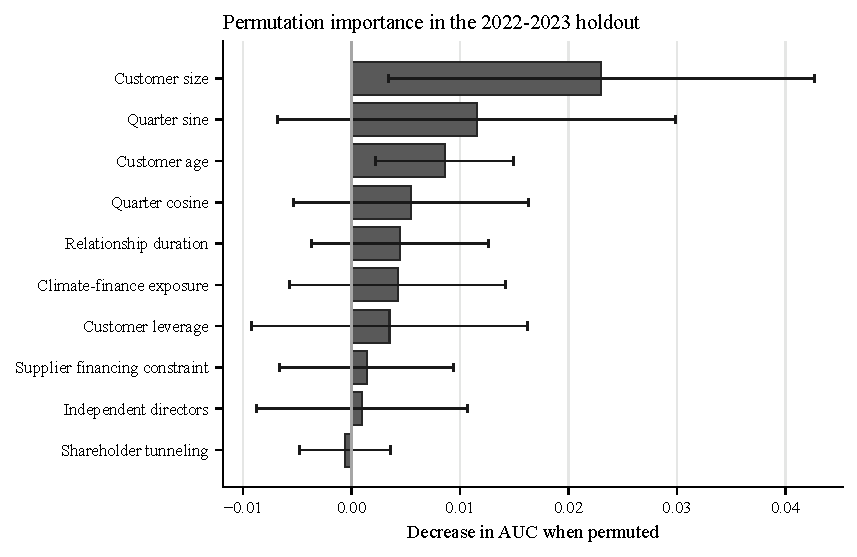
\includegraphics[width=0.86\linewidth]{../nn_supply_chain_figures/figures/fig5_permutation_importance.pdf}
\caption{Permutation feature importance, 2022--2023 holdout.
\textit{Notes}: Each bar is the mean decrease in holdout AUC when the
feature is permuted 50 times, holding all other features fixed.  Error
bars report 95\% simulation intervals across permutations.  Customer size
(C\_Size, mean AUC loss 0.023) dominates; climate-finance exposure
(Affected, 0.004) and supplier financing constraints (S\_FC, 0.001)
contribute positively but modestly.  Features with negative mean AUC loss
add no discriminative information under permutation in this sample.}
\label{fig:importance}
\end{figure}

\clearpage

\begin{figure}[H]
\centering
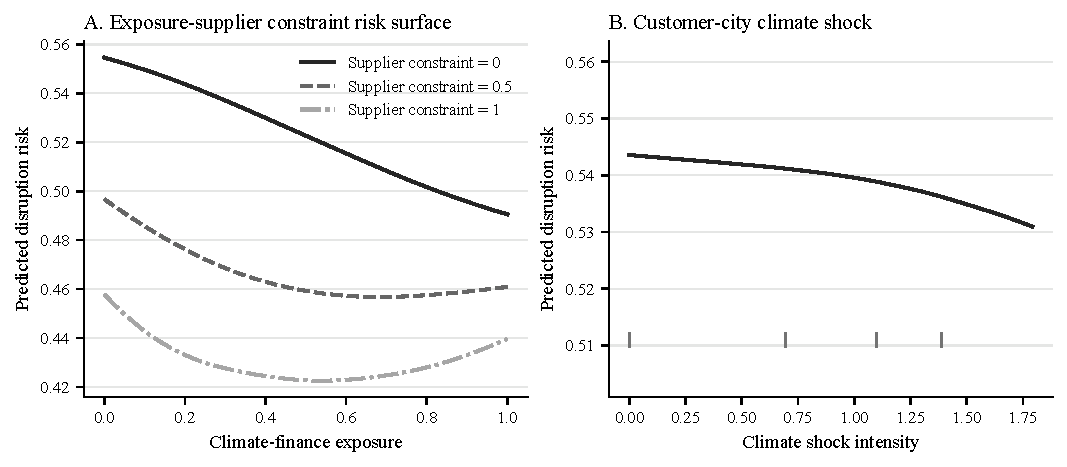
\includegraphics[width=0.98\linewidth]{../nn_supply_chain_figures/figures/fig6_risk_surface.pdf}
\caption{Model-implied supply chain risk surfaces.
\textit{Notes}: Risk surfaces average predicted disruption probabilities
over the 2022--2023 holdout covariate distribution.  Panel A varies
climate-finance exposure (Affected, $x$-axis) for three levels of
supplier financing constraints ($\textit{S\_FC} \in \{0, 0.5, 1.0\}$),
updating the interaction term consistently.  Panel B varies
customer-city climate shock intensity (Climate\_CityC); tick marks show
deciles of the empirical support.  The curves reveal nonlinear
interaction effects that linear models cannot capture without explicit
polynomial or interaction terms.}
\label{fig:surface}
\end{figure}

\end{document}
